\chapter{Eatons Method}
Turned out not to be really interesting, because it oversimplifies the rider/system interaction. Nevertheless I added it to the Davis report, because I did spend some time on it.
\section{Eaton}
In this section some identification techniques used by Eaton in order to identify the human controller will be discussed. The rider is instructed to to keep the motorcycle in a upright position and the roll angle, steering angle and steering torque are measured during the experiments. The motorcycle is observed to be a unstable system and therefore requires active control of the rider. This instablility leads to changes in the roll angle and requires corrections of the rider to keep the bike upright. The error, defined as the difference between the desired roll angle and actual roll angle, acts as an input on the rider. This error combined with the rider output (steering torque) can be used for identification purposes as Eaton demonstrates. The interesting thing about this is that Eaton uses the instability of the motorcycle to estimate the rider control, no external disturbance (altough present; i.e. unknown wind and road excitation, etc) are needed. 
\subsection{Estimating the pilot function}
Suppose you have a system according to the block diagram shown below and where the controller $C$ is subject to identification.
\begin{center}
		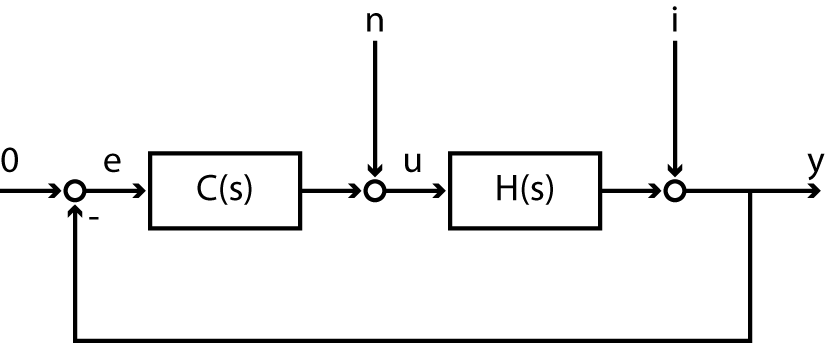
\includegraphics{images/eatonblock}
\end{center}
The system input $e$ and ouput $c$ are measurable and $n$ and $i$ represent unknown sources of noise, which are respectively defined as the remnant and external sources of disturbance.
From the block diagram we can derive that the true transferfunction is defined as:
\begin{align}
		G(s) = \frac{u(s)-n(s)}{e(s)}
\end{align}
Suppose we use the following openloop estimator to identify the transferfunction:
\begin{align}
		\hat{G(s)} = \frac{e^*(s)u(s)}{e^*(s)e(s)}
\end{align}
We get a bias in the estimate, since the noise $n$ is correlated with the error $e$. This correlation occurs because the noise is being fed back to the error. 
\begin{align}
		\hat{G(s)} = G(s) + \frac{e^*(s)n(s)}{e^*(s)e(s)}
\end{align}
However, when we assume a time delay $\tau_G(s)$ in the controller $G$, there exists a short time period where the noise is uncorrelated with the input $e$, so we can write:
\begin{align}
		\frac{e^*(s)n(s)}{e^*(s)e(s)} = 0 \ \ , \ \textrm{for; $\tau \leq \tau_G$}
\end{align}
This fact can be used to remove the bias from the signal, by making use of the physical limiations of the system and using the impulse response method. How they to this exactly remains unclear to me, additional information can be found in Eaton (1973) and in Wingrove and Edwards (1968).
\subsection{Conclusion}
The following citation is taken over from Wingrove and Edwards:
\begin{quote}
		This paper has shown that in measuring pilot describing
		functions, the identification error due to the correlation
		of the input error signal wvith the pilot's output noise can
		be reduced by shifting the input data during the computer
		analysis. The value for this time shift should be near the
		time delay of the pilot. It is shown that this idenitification
		error can be made small if the autocorrelation function
		$R_{nn}(r)$ of the internal noise source is negligible for $r$
		greater than the sum of all transport lags through the
		control loop. This means that if these conditions are met,
		it is possible to measure the describing function of a
		system with feedback, using only its own internal noise
		source for excitation.
\end{quote}
\subsection{Pros and Cons}
\begin{itemize}
		\item[+] No external perturbations required, since the instability of the machine results in a input spectrum. 
		\item[-] There is no control of the input spectrum, because it results from the rider machine interaction. This potentially could result in a limited input spectrum. However the results of Eaton show that it is possible to succesfully estimate the rider action.
		\item[-] Theory is only valid for separete rider machine systems, which are often used within McRuer theory. Unfortuneatly rider control seems to be much more interconnected with the system (multiple feedback loops, different time delays, etc).
		\item[+] The theory would be interesting to apply on the current bicycle simulator, which only makes use of visual feedback.
\end{itemize}
%\citep{wingrove2007measurement}
%\bibliographystyle{plain}
%\bibliography{articles}
